\documentclass[article]{jss}
%% -- LaTeX packages and custom commands ---------------------------------------

\usepackage{orcidlink,thumbpdf,lmodern}
\usepackage{framed}
\usepackage{amssymb}
\usepackage{amsmath}
\usepackage{hyperref}
\usepackage{dsfont}
\usepackage{enumitem}
\usepackage{graphicx}
\usepackage{float}
\usepackage[section]{placeins}

\DeclareMathOperator*{\argmin}{arg\,min}  % Define \argmin

%% new custom commands
\newcommand{\class}[1]{`\code{#1}'}
\newcommand{\fct}[1]{\code{#1()}}


%% -- Article metainformation (author, title, ...) -----------------------------

%% - \author{} with primary affiliation (and optionally ORCID link)
%% - \Plainauthor{} without affiliations
%% - Separate authors by \And or \AND (in \author) or by comma (in \Plainauthor).
%% - \AND starts a new line, \And does not.
\author{Maximilian Matthe~\orcidlink{0000-0003-0918-3766}\\Indiana University}
\Plainauthor{Maximilian Matthe}

%% - \title{} in title case
%% - \Plaintitle{} without LaTeX markup (if any)
%% - \Shorttitle{} with LaTeX markup (if any), used as running title
\title{\proglang{evomap}: A Toolbox for Dynamic Mapping in \proglang{Python}}
\Plaintitle{evomap: A Toolbox for Dynamic Mapping in Python}
\Shorttitle{evomap}

%% - \Abstract{} almost as usual
\Abstract{
  
This paper present the \pkg{evomap} package, a novel toolbox for dynamic mapping in \proglang{Python}. 
Mapping methods are essential tools for researchers across various fields to visualize relationships among
objects as spatial representations, or 'maps'. 
While existing statistical software primarily supports static mapping - analyzing relationships
at specific points in time - there's a lack of tools for exploring how these relationships change over time. 
The \pkg{evomap} package fills this gap by offering a Python implementation of the dynamic mapping framework 
EvoMap, initially proposed by \cite{Matthe+Ringel+Skiera:2023}, which extends traditional mapping methods
like Multidimensional Scaling to dynamic contexts. The package features modules for data preprocessing, 
exploration, and solution evaluation, providing a versatile toolkit for dynamic mapping applications across 
different disciplines and contexts. This paper details the foundational concepts of static and dynamic mapping
, describes the architecture and features of \pkg{evomap}, and showcases its application through an extensive 
example. }

%% - \Keywords{} with LaTeX markup, at least one required
%% - \Plainkeywords{} without LaTeX markup (if necessary)
%% - Should be comma-separated and in sentence case.
\Keywords{dynamic mapping, multidimensional scaling, proximity analysis, open-source software, \proglang{Python}}
\Plainkeywords{dynamic mapping, multidimensional scaling, proximity analysis, open-source software, Python}

%% - \Address{} of at least one author
%% - May contain multiple affiliations for each author
%%   (in extra lines, separated by \emph{and}\\).
%% - May contain multiple authors for the same affiliation
%%   (in the same first line, separated by comma).
\Address{
  Maximilian Matthe\\
  Kelley School of Business, Indiana University\\
  Department of Marketing\\
  1309 E 10th St\\ 
  47405 Bloomington, IN, USA\\
  E-mail: \email{mpmatthe@iu.edu}\\
  URL: \url{https://mpmatthe.github.io}
}

\begin{document}

%% -- Introduction -------------------------------------------------------------

%% - In principle "as usual".
%% - But should typically have some discussion of both _software_ and _methods_.
%% - Use \proglang{}, \pkg{}, and \code{} markup throughout the manuscript.
%% - If such markup is in (sub)section titles, a plain text version has to be
%%   added as well.
%% - All software mentioned should be properly \cite-d.
%% - All abbreviations should be introduced.
%% - Unless the expansions of abbreviations are proper names (like "Journal
%%   of Statistical Software" above) they should be in sentence case (like
%%   "generalized linear models" below).

\section[Introduction]{Introduction} \label{sec:intro}

Mapping, also termed 'scaling', encompasses a range of statistical methods that analyze data 
consisting of pairwise relationships using spatial representations, known as 'maps'. 
These methods map pairwise relationships onto configurations where objects are positioned 
as points within a lower-dimensional space. By employing mapping methods, 
researchers can detect underlying patterns, identify latent dimensions of 
difference.

Prominent techniques such as Multidimensional Scaling (MDS, \cite{Carroll+Arabie:1998}), 
Sammon Mapping (\cite{Sammon:1969}), or t-distributed Stochastic Neighbor Embedding 
(t-SNE, \cite{van-der-Maaten+Hinton:2008}) are extensively used across disciplines including 
statistics \citep{Saeed+etal:2019}, marketing \citep{DeSarbo+Manrai+Manrai:1994}, 
psychology \citep{Goodwill+Alasdair+Meloy:2019}, 
psychometrics \citep{Hebart+Zheng+Pereira+Baker:2020}, 
ecology \citep{Kenkel+Orloci:1986}, 
network visualization \citep{Mane+Boerner:2004}, 
and political science \citep{Jacoby+Armstrong:2014}, where they help understanding 
market competition, social network structures, ecological interactions, cognitive processes, 
latent psychological traits, or political landscapes. 

Mapping methods traditionally generate static maps based on data capturing pairwise relationships 
at a specific point in time. However, these relationships evolve due to shifts in consumer perceptions, 
social interactions, and political stances. If longitudinal data is available, it 
allows analysts to capture these dynamics, though doing so also introduces methodological challenges. 
EvoMap, as recently proposed by \citep{Matthe+Ringel+Skiera:2023}, adapts static mapping methods 
to work with longitudinal data, providing analysts with a flexible tool to harness its potential.

Thus far, however, statistical software development has focused almost entirely on static mapping. 
In \proglang{Python}, the \pkg{scikit-learn} package offers implementations of static mapping methods 
such as MDS or t-SNE \citep{Pedregosa+etal:2011}. Individual contributions exist that implement specific 
methods, such as \pkg{sammon-mapping} \citep{Perera:2023}, or \pkg{umap-learn} \citep{McInnes+Healy+Melville:2018}. 
In \proglang{R}, the \pkg{stats} package provides a function for Classical Scaling, and the \pkg{MASS} package
provides functions for Sammon Mapping and non-metric MDS \citep{Venables+Ripley:2002}. The
most comprehensive \proglang{R} package for MDS is \pkg{smacof} \citep{DeLeeuw+Mair:2009, Mair+Groenen+DeLeeuw:2022},
which implements various MDS variants and extensions. Other static mapping methods can be
found in \pkg{Rtsne} \citep{Krijthe:2015}, which implements t-SNE, or \pkg{vegan} \citep{Oksanen+etal:2022},
 \pkg{ecodist} \citep{Goslee+Urban:2007}, or \pkg{SensoMineR} \citep{Le+Husson:2008}, which implement variants of 
 non-metric MDS.

 These existing packages provide versatile toolsets for static mapping, but their functionality for dynamic mapping is 
 minimal. They provide functions that typically process only a single relationship matrix at a time. 
When analyzing a temporal sequence of matrices, such independent mapping often creates incomparable solutions that are 
challenging to compare over time \citep{Matthe+Ringel+Skiera:2023}. 
Although the \pkg{smacof} package supports three-way MDS, which allows to process multiple relationship matrices 
simultaneously, it is designed to analyze differences across individuals rather than changes over time. 
Thus, there is a clear gap in software tools dedicated to creating, exploring and evaluating dynamic maps. 

This paper presents the \proglang{Python} package \pkg{evomap}, designed to fill this gap. Developed 
as a software companion to \cite{Matthe+Ringel+Skiera:2023}, the \pkg{evomap} package provides 
a comprehensive toolbox for dynamic mapping. It offers a flexible implementation of the 
homonymous \emph{EvoMap} framework compatible with various extant static mapping methods. 
The package's modular design facilitates the addition of new mapping methods. Further, it adopts the
popular \pkg{scikit-learn} syntax, ensuring ease of use and integration into existing data analysis pipelines. 
It also includes modules for evaluation and exploration of dynamic mapping applications.

This article first provides an overview of static and dynamic mapping, essential for understanding \pkg{evomap}'s 
functionality. It then details the package's design and features, demonstrates its application through an example, 
and explores advanced considerations for practical use. The paper concludes with a discussion of
potential directions for future development.

\section{Background on Mapping} \label{sec:background}

\subsection{Static Mapping} \label{sec:static-mapping}

Static mapping positions a set of $n \in \mathbb{N}$ objects in a lower-dimensional space such that the distances among
 them closely reflect their relationships. Typically, the input data consists of a square $n \times n$ matrix of 
 pairwise relationships, usually measured as pairwise (dis-)similarities
\footnote{Although input data can vary, this discussion focuses on dissimilarities, the most prevalent type, for simplicity.}. 
The outcome is an $n$-point configuration in $d \in \mathbb{N}$ dimensions, typically visualized as a two-dimensional 
'map' \citep{Borg+Groenen:2005}. To enhance interpretability, one can augment the maps by incorporating additional 
features of the analyzed objects, for instance, via property fitting \citep{DeSarbo+Hoffman:1987} or by binding them to 
visual elements like the size or color of each point \citep{Ringel+Skiera:2016}.

Mapping originated in Psychometrics with Torgerson's Classical Scaling \cite{Torgerson:1958}. Since then, research from 
different fields has developed several variants. For instance, \cite{Shepard:1962a, Shepard:1962b} introduced monotonic 
transformations of the input dissimilarities, leading to non-metric MDS \citep{Kruskal:1964a, Kruskal:1964b}. Other 
extensions process measurements from multiple subjects \citep{Carroll+Chang:1970} or link the input dissimilarities to 
map distances using non-linear functions \citep{Sammon:1969}. More recently, other fields, like computer science have 
contributed methodological innovations, such as t-SNE \citep{van-der-Maaten+Hinton:2008}.

Commononly, these methods fit point coordinates $\hat{X} \in \mathbb{R}^{n \times d}$ of $n$ objects to 
given data by minimizing the discrepancy between map distances and input dissimilarities. For MDS, this 
discrepancy is measured through the Stress function:

\begin{equation} \label{eq:stress}
  Stress(X) = \sqrt{\frac{\sum_{i,j}(d(x_i, x_j) - \hat{d}_{ij})^2}{\sum_{i,j}d(x_i, x_j)^2}},
\end{equation}

where $d(x_i, x_j)$ and $\hat{d}_{i,j}$ denote the map distances and input dissimilarities among objects i and j, respectively 
(or, depending on the MDS variant, a transformation thereof).

\begin{equation} \label{eq:xhat}
  \hat{X} = \argmin_{X \in \mathbb{R}^{n \times d}} \text{Stress}(X),
\end{equation}

The quality of $\hat{X}$ can be evaluated in multiple ways, including the Stress value, different agreement metrics 
like the Hit-Rate of K-nearest neighbor recovery \cite{Chen+Buja:2009}, or through visual comparisons, like the 
Shepard Diagram.  

\begin{figure}
  \centering
  \resizebox{\textwidth}{!}{\includegraphics{../gen/Fig1_static_mapping.png}}
  \caption{\label{fig:static-map} Illustration of Static Mapping}
\end{figure}
  
Figure \ref{fig:static-map} illustrates non-metric MDS applied to technology firms based on the
textual similarity of their product descriptions in 1998, using data from the TNIC dataset \citep{Hoberg+Phillips:2016}.
The map (left) reveals that, within the nine depicted firms, there are four 
groups of similar firms based on their main products sold in 1998: i) hardware-focused firms, such
as Apple, Western Digital, and Micron Technologies; ii) platform-focused firms, like Microsoft and
Oracle, iii) software-focused firms, such as eBay and Intuit, and iv) telecommunication service
providers, like AT\&T and US Cellular. Among these pairs, the telecommunication firms appear
more distinct compared to the remaining groups whose products commonly relate to computers.
Within the three computer-related groups, Microsoft and Oracle, known for platforms like the
Windows Operation System or Oracle’s Database System, appear between software and hardware
providers. Among the hardware providers, Micron Technologies, primarily known as a
semiconductor firm, is differentiated from Western Digital, known for storage solutions, 
and Apple, known for personal computers like the iMac.

The Shepard Diagram (right) confirms the map's good solution quality. The transformed
dissimilarities fit the observed input dissimilarities well, and the rank correlation between the
observed input dissimilarities and the map distances remains high at .84. 

As firms change their relative positions over time, a map of the same firms generated 
at different points in time would likely look different. If longitudinal measurements are
available, the analyst could track the evolution of these maps, gaining insights into the timing, extend, and 
duration of changes. These are precisely the insights dynamic mapping seeks to provide.

\subsection{Dynamic Mapping} \label{sec:dynamic-mapping}

Dynamic mapping extends static mapping by revealing how relationships among $n$ objects change over time. 
In dynamic mapping, the input data consist of a sequence of relationship matrices $(D_t)_{t=1, \dots, T}$
 rather than a single matrix.  
Applying static mapping methods to each time-point matrix independently, $D_t$, introduces several issues. 
The estimated point configurations $(\hat{X}_t)_{t=1, \dots, T}$, where $X_t \in \mathbb{R}^{n \times d}$, do 
not align over time. Additionally, results can be inconsistent due to local optima and are highly sensitive to 
variations in the data, including noise.

\emph{EvoMap}, as proposed by \cite{Matthe+Ringel+Skiera:2023}, addresses these issues 
by incorporating static mapping methods into a dynamic optimization framework. 
\emph{EvoMap} jointly fits a sequence of point configurations $(\hat{X}_t)_{t=1,\dots,T}$
to a sequence of dissimilarity matrices $(D_t)_{t=1,\dots,T}$, linking them over time 
through a regularization component. Thereby, it not only aligns subsequent maps 
but also smooths the trajectories of objects on the map. As a result, 
 \emph{EvoMap} produces coherent spatial representations of the evolving relationships 
 among the objects under analysis (“dynamic maps”).

Specifically, \emph{EvoMap}’s optimization problem is defined as:

\begin{equation} \label{eq:evomap-optim}
  (\hat{X}_t)_{t=1,\ldots,T} = \argmin_{X_1, \ldots, X_T \in \mathbb{R}^{n \times d}} C_{total}(X_1, \ldots, X_T),
\end{equation}

with the total cost function:

\begin{equation} \label{eq:cost-total}
  C_{total}(X_1, \ldots, X_T) = \sum_{t=1}^T{C_{static}(X_t)} + \alpha \cdot C_{temporal}(X_1, \ldots, X_T),
\end{equation}

Here, $C_{static}$ represents the static component of EvoMap’s cost function, which equals
the sum of the cost function $C_{static}$ of the selected static mapping method evaluated at each period
$t \in \{1, \ldots, T\}$. When paired with MDS, for instance, $C_{static}$ would equal the Stress function in
equation \ref{eq:stress}. $C_{temporal}$, controlled by the hyperparameter $\alpha \in \mathbb{R}$, represents the temporal component of the cost function, which
aligns the maps and smooths objects’ movements over time. The temporal cost component, $C_{temporal}$, is
further defined as:

\begin{equation} \label{eq:cost-temporal}
  C_{temporal}(X_1, \ldots, X_T) = \sum_{i=1}^n{f_w(i)} \sum_{k=1}^p \sum_{t=k=1}^T \mathds{1}_{\{i \in I\}} \left\| \nabla^k x_{i,t} \right\|^2,
\end{equation}

where \\
\begin{description}
  \item $\mathds{1}_{\{i \in I_{t,k}\}}: I \rightarrow \{0,1\}$ denotes an indicator function equal to one if firm \\
   $i$ is present in time $t$ and the $k$ preceding periods: \\
  $\mathds{1}_{\{i \in I_{t,k}\}} := \prod_{l=0}^k \mathds{1}_{\{i \in I_{t-l}\}}$, \\
  \item $f_w : I \rightarrow \mathbb{R}^+$ is a positive weight function defined over the set of firms $I$, \\
  \item $p \in \mathbb{N}$ is a second hyperparameter of positive integer values that controls the degree of \\ 
  smoothing, and \\
  \item $\nabla^kx_{i,t} \in \mathbb{R}^d$ is the k-th (backward) difference of firm $i$’s map position at time $t$. \\ 
  We refer to \cite{Matthe+Ringel+Skiera:2023} for more details and intuition on \emph{EvoMap}'s cost function.
\end{description}

Figure \ref{fig:dynamic-map-illustration} demonstrates dynamic mapping for nine technology firms over 20 years, 
contrasting a static 1998 snapshot (left) with their evolving positions (right). The dynamic map, 
created by applying \emph{EvoMap} to 20 dissimilarity matrices, reveals how the firms' positions evolved over time. 
Apple and Western Digital, for instance, part ways as Apple ventures into the software space - bringing it closer to firms like Intuit. 
Microsoft and Oracle converge further, while the telecommunication firms’ positions
remain static in comparison. In its remainder, this paper details how to create dynamic maps
 using the \pkg{evomap} package.

\begin{figure}
  \centering
  \resizebox{\textwidth}{!}{\includegraphics{../gen/Fig2_dynamic_mapping.PNG}}
  \caption{\label{fig:dynamic-map-illustration} Illustration of Dynamic Mapping}
\end{figure}

\section[The evomap Package]{The \pkg{evomap} Package} \label{sec:package}

\subsection{Installation}

The \pkg{evomap} package is accessible for installation directly from GitHub. Users can install it using the following
 command in the terminal:

\begin{CodeChunk}
  \begin{CodeInput}
  > pip install git+https://github.com/mpmatthe/evomap
  \end{CodeInput}
\end{CodeChunk}

The installation requires \proglang{Python} version 3.7.1 or
newer, alongside an operational \proglang{C} compiler. At the time of writing the latest release of \pkg{evomap} is 
version 0.2.0. Updates are actively developed on GitHub, available at \href{https://github.com/mpmatthe/evomap} 
{https://github.com/mpmatthe/evomap}. Future versions will be released as pre-compiled packages through the Python 
Package Index (PyPi) for easy access.

\subsection{Dependencies}

The \pkg{evomap} package draws on a limited number of other packages. It relies on \pkg{numpy} and \pkg{scipy} for 
numerical computations and \pkg{matplotlib} and \pkg{seaborn} for plotting. To optimize runtime, individual functions 
are either precompiled to \proglang{C} using \pkg{cython}, or use the just-in-time \proglang{C}-compiler \pkg{numba}.

\subsection{Package Overview}

The \pkg{evomap} package is structured into six key modules\footnote{For clarity, the unified term 'module' encompasses 
submodules, modules, and subpackages.}, designed to streamline the analysis workflow:

\vbox{%
\begin{enumerate}
  \item \code{datasets}: Offers example datasets, enabling users to familiarize themselves with the package's %
  capabilities. 
  \item \code{preprocessing}: Transforms diverse input data into a format compatible with EvoMap. 
  \item \code{mapping}: Contains EvoMap implementations for various static mapping methods, allowing users to apply % 
  EvoMap to their data.
  \item \code{printer}: Provides tools for visual exploration of both static and dynamic mapping results. 
  \item \code{transform}: Includes options for map adjustments (e.g., rotations and reflections) that can enhance %
  interpretability. 
  \item \code{metrics}: Features a suite of evaluation metrics and goodness-of-fit statistics to evaluate mapping %
  results. 
\end{enumerate}}

Table \ref{tab:modules} presents an overview of these modules, with detailed descriptions and complete API 
references available at \href{https://evomap.readthedocs.io/en/latest/autoapi/evomap/index.html} {ReadTheDocs}.

 \begin{table}[hbt!]
  \centering
  \begin{tabular}{p{.5cm}p{4.25cm}p{4.25cm}p{4.25cm}}
  \hline
  \# & Name & Purpose & Exemplary Functions or Classes\\ 
  \hline
  (1) & evomap.datasets       & Load exemplary datasets \newline                  & \code{load\_tnic\_snapshot()} \\
  (2) & evomap.preprocessing  & Prepare data for mapping \newline \newline        & \code{coocc2sim()}, \code{edgelist2matrix()} \\ 
  (3) & evomap.mapping        & Apply EvoMap to data \newline                     & \code{MDS()}, \code{EvoMDS()}, \code{TSNE()}, \code{EvoTSNE()}\\
  (4) & evomap.printer        & Visualize mapping results \newline                & \code{draw\_map()}, \code{draw\_dynamic\_map()}, \code{draw\_map\_sequence()}\\ 
  (5) & evomap.transform      & Adjust mapping results \newline for easier interpretation \newline   & \code{align\_map()} \\
  (6) & evomap.metrics        & Assess mapping quality  \newline                  & \code{misalign\_score()}, \code{hitrate\_score()}, \code{persistence\_score()}\\
  \hline
  \end{tabular}
  \caption{\label{tab:modules} Overview of modules.}
  \end{table}
  
\subsection{Basic Usage} 

The primary use case for \pkg{evomap} is transforming longitudinal relationship data into dynamic low-dimensional 
spatial representations. The process is straightforward and involves the following three steps:

\begin{enumerate}
  \item \textbf{Import the EvoMap class} for the desired mapping method.
  \item \textbf{Initialize EvoMap} with appropriate parameters.
  \item \textbf{Fit EvoMap} to your data using \code{fit_transform()}.
\end{enumerate}

For example, consider longitudinal data represented by a sequence of 20 dissimilarity matrices for 9 firms, each stored as a
\pkg{numpy} array \code{D_t} of shape \code{(9,9)}.

\begin{CodeChunk}
\begin{CodeInput}
>>> print(len(D_t))       # Output: 20
>>> print(D_t[0].shape)   # Output: (9,9)
\end{CodeInput}
\end{CodeChunk}

To apply non-metric MDS, instantiate \code{EvoMDS()}, specify the \code{mds\_type} as \code{'ordinal'}, 
set its hyperparameters $\alpha$ and $p$ (whose role we detail later), and initial starting positions. Then, fit 
EvoMap to your data: 

\begin{Code}
>>> from evomap.mapping import EvoMDS   
>>> evomds = EvoMDS(
...     alpha=.2, 
...     p=2, 
...     mds_type='ordinal', 
...     init=cmds_t)                  
>>> X_t = evomds.fit_transform(D_t)  
\end{Code}

The result, \code{X_t}, is a sequence of \code{numpy} arrays,  
mapping the firms onto two dimensions over 20 years. 

\begin{CodeChunk}
\begin{CodeInput}
>>> print(len(X_t))   # Output: 20
>>> print(X_t[0].shape)   # Output: (9,2)   
\end{CodeInput}
\end{CodeChunk}

To explore the result, visualize the point coordinates stored in \code{X_t} with \code{draw_dynamic_map()},
providing labels, and optionally displaying arrows and axes. Figure \ref{fig:dynamic-map} showcases the resultant 
evolution of the nine firms' positions from 1998 to 2017. 

\vbox{
\begin{CodeChunk}
\begin{CodeInput}
>>> from evomap.printer import draw_dynamic_map
>>> draw_dynamic_map(
...     X_t, 
...     label=labels, 
...     show_arrows=True, 
...     show_axes=True)  
\end{CodeInput}
\end{CodeChunk}    
}

\begin{figure}
  \centering
  \resizebox{0.5\textwidth}{!}{\includegraphics{../gen/Fig3_dynamic_map.PNG}}
  \caption{\label{fig:dynamic-map} Dynamic Map of Nine Technology Firms, 1998 - 2017.}
\end{figure}

The \pkg{evomap} package encompasses a full toolbox of functionalities beyond simply generating dynamic maps. 
It equips users with a range of tools for each step of the data analysis process, from initial data preprocessing 
and formatting to the exploration and assessment of the mapping results. The following section briefly illustrates 
the overall package design and implementation, before the paper delves into a more comprehensive usage example. 

\subsection{Package Design and Implementation}

The \pkg{evomap} package is centered around its \code{mapping} module. This module is the heart of \pkg{evomap}, 
implementing the \emph{EvoMap} framework for various mapping methods along with their optimization routines. 
As detailed in section \ref{sec:dynamic-mapping}, \emph{EvoMap}’s cost function contains a static and a temporal 
component - the former varies by mapping method, while the latter is consistent across all \emph{EvoMap} implementations. 
Accordingly, the \code{mapping} module follows a dual structure as well. There, a static implementation
of each mapping method provides its static cost component, while a dynamic implementation integrates the method
into the \emph{EvoMap} framework. For MDS, for instance, the \code{mapping} module includes \code{MDS} (static)
 and \code{EvoMDS} (dynamic). 

This dual structure enables users to employ mapping methods in both static and dynamic contexts. More importantly, 
it provides a modular structure than can easily be extended to incorporate new mapping methods. To add a new method, 
one must only introduce a static class defining the static cost function and a new instance of the 
EvoMap \code{core} interface. Figure \ref{fig:package-design} visualizes the package architecture and highlights this 
modularity. Common functionalities are provided by dedicated classes, such as \code{optim} or \code{core}, and 
shared across implementations. As a result, extending the framework is easy, and all enhancements to the core 
framework affect all mapping implementations uniformly.

\begin{figure}[hbt!]
  \centering
  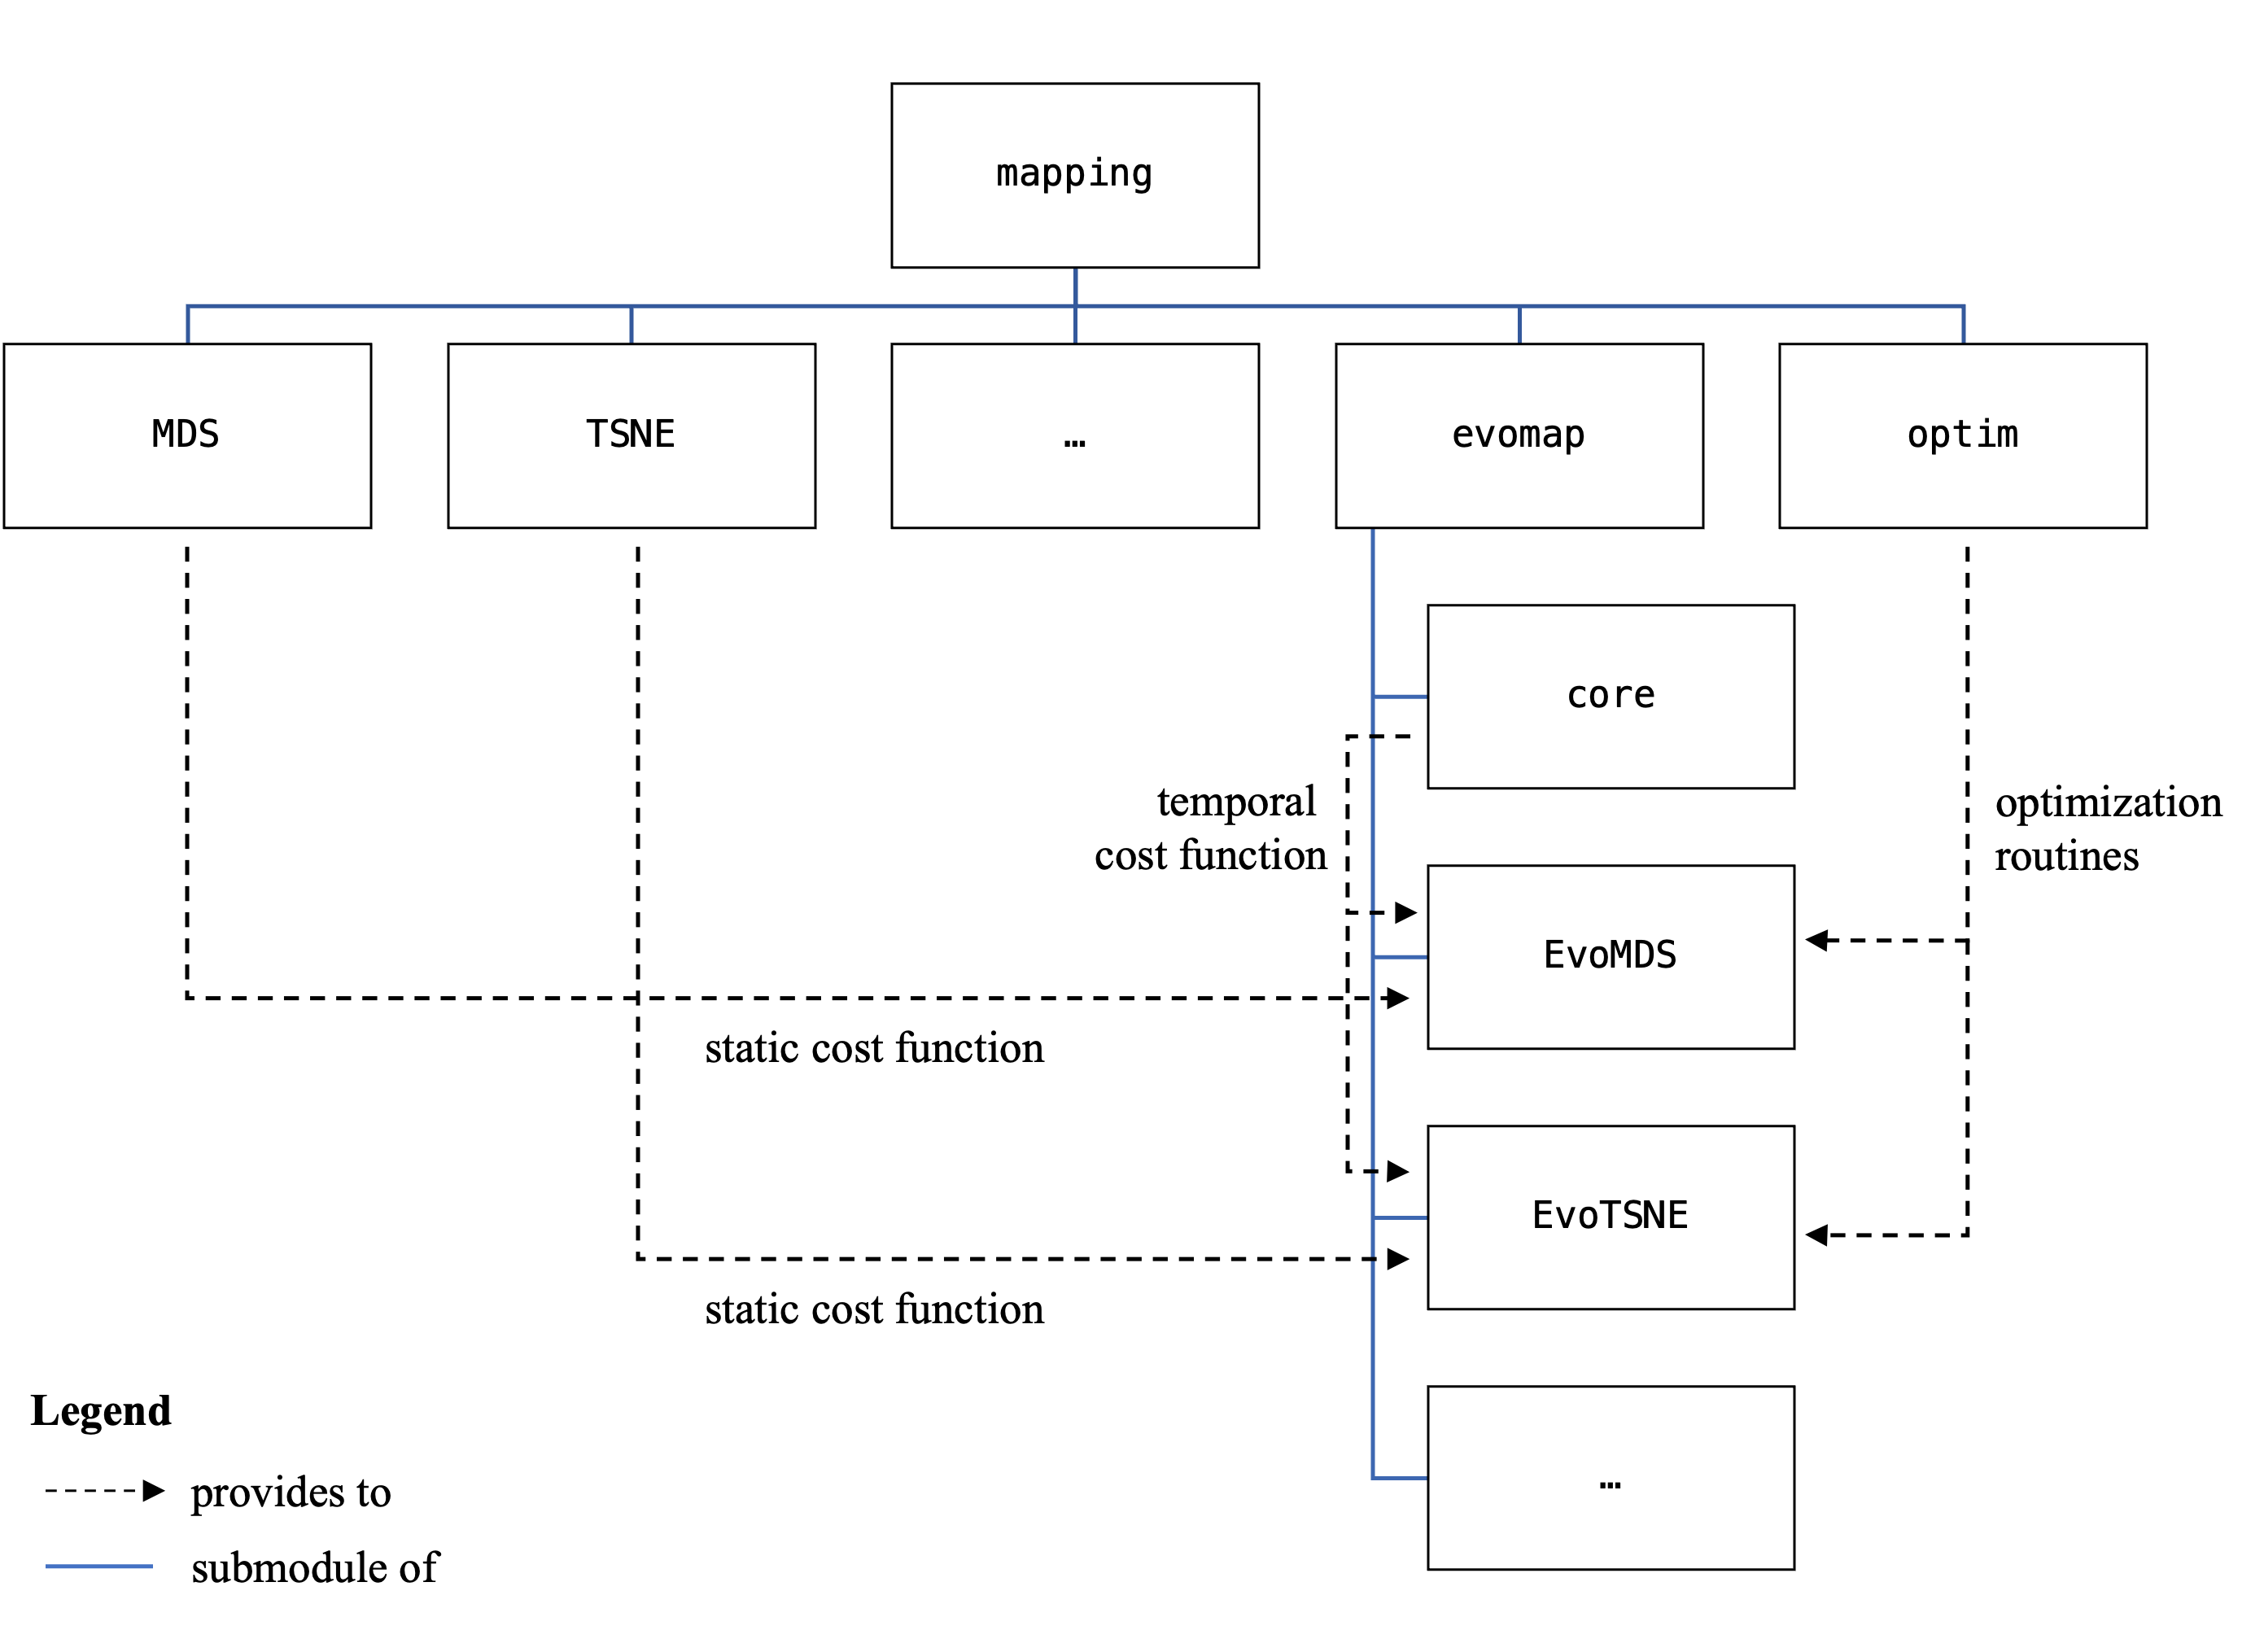
\includegraphics{../misc/package-design.png}
  \caption{\label{fig:package-design} Overview of the Mapping Module.}
\end{figure}
  
Currently, \pkg{evomap} provides implementations for three mapping methods (MDS, Sammon
Mapping, t-SNE), which can serve as blueprints for future extensions. Having presented the
general design and structure of the package, the next section illustrates its practical usage. 

%% -- Detailed Usage Example -------------------------------------------

\section{Detailed Usage Example} \label{sec:usage-example}

This section demonstrates how to apply the \pkg{evomap} package to a subset 
of the Text-based Network Industries Classification (TNIC) dataset by \cite{Hoberg+Phillips:2016}. 
It provides a step-by-step guide, showcasing the tools within \pkg{evomap} that facilitate 
each phase of the analysis. 

The TNIC dataset captures firm-firm relationships based on the linguistic similarity of their product descriptions 
in annual reports. The small subset used for this illustration focuses on nine technology companies: 
Apple, AT\&T, eBay, Intuit, Micron Technology, Microsoft, Oracle, US Cellular, and Western Digital, 
spanning twenty years from 1998 to 2017. Each data point represents a pair of firms at a given time, 
including their names, a similarity score, Standard Industrial Classification (SIC) codes, 
and a size variable derived from their market values. To load this subset, run:

\begin{Code}
>>> from evomap.datasets import load_tnic_sample_tech
>>> data = load_tnic_sample_tech()
\end{Code}

Table \ref{tab:data-overview} lists the first and last five rows to illustrate the data structure. 
Each row details the year, firm names (name1, name2), their pairwise similarity score, SIC codes (sic1, sic2), and size
 variables (size1, size2).

\begin{table}[t!]
  \centering
  \begin{tabular}{ccp{3cm}p{3cm}cccccc}
  \hline
  row & year & name1 & name2 & score & sic1 & sic2 & size1 & size2 \\ 
  \hline
  0 & 1998 & APPLE INC & WESTERN DIGITAL CORP & 0.0657 & 36 & 35 & 71.79 & 32.29 \\
  1 & 1998 & APPLE INC & MICROSOFT CORP & 0.0601 & 36 & 73 & 71.79 & 517.38 \\
  2 & 1998 & APPLE INC & ORACLE CORP & 0.0355 & 36 & 73 & 71.79 & 188.44 \\
  3 & 1998 & AT\&T INC & US CELLULAR CORP & 0.0761 & 48 & 48 & 324.14 & 57.62 \\
  4 & 1998 & EBAY INC & MICROSOFT CORP & 0.0281 & 73 & 73 & 98.54 & 517.38 \\
  \vdots & \vdots & \vdots & \vdots & \vdots & \vdots & \vdots & \vdots & \vdots \\
  437 & 2017 & ORACLE CORP & MICROSOFT CORP & 0.1292 & 73 & 73 & 432.13 & 728.91 \\
  438 & 2017 & ORACLE CORP & INTUIT INC & 0.0231 & 73 & 73 & 432.13 & 187.30 \\
  439 & 2017 & US CELLULAR CORP & AT\&T INC & 0.0184 & 48 & 48 & 56.56 & 488.57 \\
  440 & 2017 & WESTERN DIGITAL CORP & APPLE INC & 0.0321 & 35 & 36 & 161.40 & 888.85 \\
  441 & 2017 & WESTERN DIGITAL CORP & MICRON TECHNOLOGY INC & 0.0788 & 35 & 36 & 161.40 & 188.55 \\
  \hline
  \end{tabular}
  \caption{Overview of the TNIC Sample Data} \label{tab:data-overview}
\end{table}
  
\subsection{Preprocessing}

The \pkg{evomap} package is designed to analyze longitudinal relationship data, requiring input as 
a sequence of $n \times n$ relationship matrices, where $n$ represents the number of objects. 
These matrices should contain non-negative real numbers, typically representing similarities or dissimilarities. 
Each matrix should be symmetric, normalized (usually between 0 and 1), and free of missing values. 
The dataset should be balanced, with a consistent set of objects across time. 
A later section shows how to handle unbalanced data as well.

Many mapping methods, like MDS, require dissimilarities as their input. When the available data 
does not directly fit this requirement, \pkg{evomap} offers preprocessing functions to convert various 
data types into a suitable format. 

For the TNIC example, which is initially provided as a time-indexed edgelist and measures 
similarities rather than dissimilarities, the first step involves converting the edgelist 
into a sequence of matrices. This is achieved using the \code{edgelist2matrices()} function,
specifying columns for object identifiers, similarity scores, and time indicators. 

\begin{Code}
>>> from evomap.preprocessing import edgelist2matrices
>>> S_t, labels_t = edgelist2matrices(
...     data,
...     score_var='score',
...     id_var_i='name1',
...     id_var_j='name2',
...     time_var='year')  
\end{Code}

The next step involves converting similarity measures into dissimilarities. 
This can be done through a straightforward transformation, $diss_{i,j} = 1 - sim_{i,j}$, which, alongside 
other transformations, is available in the \code{sim2diss()} function. 
We apply this transformation to each matrix in the series, which yields a list of 20 dissimilarity matrices, 
each of shape $(9,9)$, ready for dynamic mapping with EvoMap.

\begin{Code}
>>> from evomap.preprocessing import sim2diss
>>> D_t = [sim2diss(S, transformation = 'mirror') for S in S_t]
\end{Code}
  
\subsection{Dynamic Mapping with EvoMap}

Dynamic mapping with EvoMap involves initializing the desired mapping method and executing the \code{fit_transform()} 
function. EvoMap then transforms the preprocessed dissimilarity matrices into dynamic maps that represent the evolving 
relationships among objects over time. For example, to use EvoMDS for Multidimensional Scaling, run:

\begin{Code}
>>> evomds = EvoMDS(
...     alpha=0.2, 
...     p=2, 
...     mds_type='ordinal', 
...     init=cmds_t)                  
>>> X_t = evomds.fit_transform(D_t)    
\end{Code}

Key parameters to consider when initializing EvoMap include:
\begin{itemize}
  \item \textbf{EvoMap's Hyperparameters:} These include $\alpha$ and $p$, which regulate the degree of alignment and smoothness.
  \item \textbf{Method-Specific Arguments:} These vary by the mapping method used. For instance, \code{mds_type} %
  specifies the type of MDS (e.g., ratio, interval, or ordinal), while \code{perplexity} determines how closely or %
  broadly t-SNE groups data points together. 
  \item \textbf{Starting Positions:} The initial configuration, \code{init}, which can significantly influence the optimization process and final % 
  mapping quality. 
  \item \textbf{Optimization Arguments:} These impact convergence and computational time. For example, \code{n_iters}, %
  which sets the number of iterations for the optimization algorithm.  
\end{itemize}

The following sections outline these choices in more detail. 

\subsubsection{Starting Positions}

To achieve consistent results across different runs, it's important to control the initialization of the optimization 
process. This can be done in two ways:

\begin{enumerate}
    \item \textbf{Setting a Fixed Seed:} Use \code{np.random.seed()} with a specific number before instantiating EvoMap to %
    ensure random initializations are reproducible.
    \item \textbf{Setting Starting Positions:} Use the \code{init} argument to provide predetermined starting positions when %
    instantiating EvoMap.
\end{enumerate}

The \code{init} parameter accepts a list of starting positions matching the desired output shape, in this case, 
\code{(9,2)}. A common strategy is to use the output of another mapping method, such as Classical Scaling, for 
these starting positions. This approach can potentially lead to a solution with lower stress when applying MDS 
\citep{DeLeeuw+Mair:2009}.

In our example, we employ the Classical Scaling solution from the first time period as the starting positions for all 
periods. Classical Scaling is fully deterministic, does not rely on random seeds, and offers full reproducibility. 
Classical Scaling can be applied via \code{CMDS} in \code{evomap.mapping}, similar to other 
mapping methods, by using \code{fit\_transform()}. Using \code{CMDS}, we generate a list of identical starting positions 
for each period:

\begin{CodeChunk}
\begin{CodeInput}
>>> from evomap.mapping import CMDS
>>> cmds_t = []
>>> cmds = CMDS().fit_transform(D_t[0])
>>> for t in range(n_periods):
...     cmds_t.append(cmds)
\end{CodeInput}
\end{CodeChunk}

\subsubsection{Hyperparameters in Dynamic Mapping}

\emph{EvoMap} requires the user to set two hyperparameters: $\alpha$ and $p$. 
$\alpha$ influences how strongly subsequent point coordinates align with each other, 
whereas $p$ controls the smoothness of each object's movement path across time. Carefully selecting
these hyperparameters is crucial, as they strongly affect EvoMap's output. 

Users of the \pkg{evomap} package can identify suitable values for $\alpha$ and $p$ in two primary ways: 

\begin{enumerate}
  \item \textbf{Visual Inspection:} Explore EvoMap's output under various hyperparameter combinations. 
  \item \textbf{Quantitative Evaluation:} Use a grid search to systematically test and evaluate a range of %
  hyperparameter combinations.
\end{enumerate}

To demonstrate the influence of these hyperparameters, we examine the effects of different $\alpha$ and $p$ 
values on EvoMap's output using the TNIC dataset as an example. Figure \ref{fig:hyperparameters} displays 
dynamic mapping results generated with different hyperparameter choices, showcasing how each parameter alters the mapping 
results. The first row varies $\alpha$ (holding $p$ constant at 1), the second row varies $p$ (holding $\alpha$ constant
at a medium value).

\begin{figure}[hbt!]
  \centering
  \resizebox{\textwidth}{!}{\includegraphics{../gen/Fig5_hyperparamters.png}}
  \caption{\label{fig:hyperparameters} Dynamic Map Under Different Hyperparameter Choices.}
\end{figure}
  
Figure \ref{fig:hyperparameters} illustrates that a lower $\alpha$ value tends to produce maps with weaker alignment 
and more erratic movement paths. As $\alpha$ increases, maps become more aligned, and the movement paths shorten. 
An excessively high $\alpha$ might lead to nearly static maps, showing only minimal changes over time. 
Conversely, the impact of $p$ is less about the length of the paths and more about their smoothness; higher $p$ values 
decrease zigzag movements, leading to smoother trajectories and more uniform distances between subsequent points.

A later section will discuss a methodological approach, a grid search, for selecting appropriate 
values for $\alpha$ and $p$.

\subsubsection{Convergence Diagnostics}

\pkg{evomap} operates quietly by default, providing no details about the convergence
of its gradient-based optimization. However, such information on convergence can be crucial, 
especially when faced with suboptimal solution quality or unexpected results. 
To obtain such diagnostics, users can modify the \code{verbose} parameter to increase output verbosity: 
\begin{itemize}
  \item \code{verbose=1} (the default) means no output is provided.
  \item \code{verbose=2} reveals basic information about the optimization routine, the final cost function value, and % 
  convergence status.
  \item \code{verbose=3} offers detailed insights into the optimization process, including cost function values at %
  specific intervals.  
\end{itemize}

Setting \code{verbose = 1}, for instance, indicates the optimization routine (gradient descent with backtracking)
and an indication of its successful convergence at iteration 105:

\begin{CodeChunk}
\begin{CodeInput}
>>> EvoMDS(
...   alpha=.2,
...   mds_type='ordinal',
...   init=cmds_t,
...   verbose=1
... ).fit(D_t)    
\end{CodeInput}
\begin{CodeOutput}
[EvoMDS] Running Gradient Descent with Backtracking via Halving
[EvoMDS] Iteration 105: gradient norm vanished. Final cost: 3.80
\end{CodeOutput}
\end{CodeChunk}

Here, we use \code{fit()}, which runs EvoMap without returning the resultant point coordiantes. 
Setting \code{verbose=2} and \code{n_iter_check=20} evaluates the cost function every 20 iterations and reveals 
how the cost function values decrease monotonically, until the gradient norm vanishes around iteration 105.

\begin{CodeChunk}
\begin{CodeInput}
>>> EvoMDS(
...     alpha=.2,
...     mds_type='ordinal',
...     init=cmds_t,
...     n_iter_check=20,
...     verbose=2
... ).fit(D_t)    
\end{CodeInput}
\begin{CodeOutput}
[EvoMDS] Running Gradient Descent with Backtracking via Halving
[EvoMDS] Iteration 20 -- Cost: 3.81 -- Gradient Norm: 0.0245
[EvoMDS] Iteration 40 -- Cost: 3.80 -- Gradient Norm: 0.0104
[EvoMDS] Iteration 60 -- Cost: 3.80 -- Gradient Norm: 0.0076
[EvoMDS] Iteration 80 -- Cost: 3.80 -- Gradient Norm: 0.0058
[EvoMDS] Iteration 100 -- Cost: 3.80 -- Gradient Norm: 0.0012
[EvoMDS] Iteration 105: gradient norm vanished. Final cost: 3.80
\end{CodeOutput}
\end{CodeChunk}

Should these diagnostics indicate issues with convergence, several strategies can help improve optimization performance.
Specifically, the user can:

\vbox{
\begin{itemize}
  \item Utilize \code{evomap.preprocessing} to normalize input data, as some \\ 
  mapping methods struggle with input data measured on unusual or very large scales.
  \item Increase \code{n_iter} to extend the number of allowed iterations.
  \item Adjust \code{step_size} (by default: 1) to modify convergence speed; decrease if optimization overshoots, or \\ 
  increase it for faster convergence. 
  \item Experiment with multiple initializations through \code{n_inits} to mitigate the impact \\
  of random starting positions. 
\end{itemize}
}

Once the user is confident about proper convergence of the optimization, one can start exploring
the results in more depth and evaluate the solution quality more rigorously.

\subsection{Exploration}

The \pkg{evomap} package provides a range of options to explore mapping results visually through the \code{printer}
module. One can categorize these functions into two groups:

\begin{enumerate}
  \item \textbf{Static Maps:} visualizing individual snapshots at a time
  \item \textbf{Dynamic Maps:} visualizing the evolution over time. 
\end{enumerate}

\subsubsection{Static Maps}

Static snapshots help evaluate the quality of mapping solutions and set reference points
for dynamic exploration. The primary function for static visualization is \code{draw_map()},
which, in its simplest form, requires just the point coordinates $\hat{X}$ to generate a scatter plot. 
For unidimensional data, it plots a line scale. Figure \ref{fig:static-snapshots} displays three examples of static 
snapshots.

\begin{CodeChunk}
\begin{CodeInput}
>>> fig, ax = plt.subplots(1,3)
>>> draw_map(X_t[0], label=labels, ax=ax[0])
>>> draw_map(X_t[10], label=labels, ax=ax[1])
>>> draw_map(X_t[19], label=labels, ax=ax[2])
\end{CodeInput}
\end{CodeChunk}

\begin{figure}[hbt!]
\centering
\resizebox{\textwidth}{!}{\includegraphics{../gen/Fig6_static_snapshots.png}}
\caption{\label{fig:static-snapshots} Three Static EvoMap Snapshots}
\end{figure}  

Further customization is possible by binding additional information about each object to the map's aesthetics, 
such as labels, colors, and sizes, as illustrated in 
Figure \ref{fig:draw-map-illustrations}. 

\vbox{
\begin{CodeChunk}
\begin{CodeInput}
>>> draw_map(X_t[0])
>>> draw_map(X_t[0], label=labels)
>>> draw_map(X_t[0], label=labels, color=sic_codes)
>>> draw_map(X_t[0], label=labels, color=sic_codes, size=sizes)
\end{CodeInput}
\end{CodeChunk}
}

\begin{figure}[hbt!]
  \centering
  \resizebox{0.7\textwidth}{!}{\includegraphics{../gen/Fig7_draw_map_illustrations.png}}
  \caption{\label{fig:draw-map-illustrations} Static Map with Different Aesthetics.}
\end{figure}
  
\subsubsection{Dynamic Maps}

Beyond individual snapshots, \pkg{evomap} allows to create dynamic maps, 
overlaying multiple snapshots to illustrate changes over time. 
This is accomplished with \code{draw_dynamic_map()} or \code{draw_trajectories()}.

Dynamic maps incorporate the same aesthetic customizations as static maps but extend them to reflect changes 
across time points. Thus, variables like color or size should be provided as lists of arrays, each corresponding
 to a specific time point.

An example of creating a dynamic map with additional aesthetics is:

\begin{CodeChunk}
\begin{CodeInput}
>>> from evomap.printer import draw_dynamic_map
>>> draw_dynamic_map(X_t,
...     label=labels,
...     color_t=sic_codes_t,
...     size_t=sizes_t,
...     show_arrows=True,
...     show_axes=True,
...     title='A: Dynamic Map')  
\end{CodeInput}
\end{CodeChunk}

To focus solely on the movement paths, \code{draw_trajectories()} 
offers a specialized view highlighting the trajectory of each object through time.

\begin{CodeChunk}
\begin{CodeInput}
>>> from evomap.printer import draw_trajectories
>>> draw_trajectories(X_t,
...     labels=labels,
...     period_labels=periods,
...     show_axes=True,
...     title='B: Trajectories')  
\end{CodeInput}
\end{CodeChunk}

\begin{figure}[hbt!]
  \centering
  \resizebox{0.7\textwidth}{!}{\includegraphics{../gen/Fig8_dynamic_map_and_trajectories.png}}
  \caption{\label{fig:draw-dynamic-map-and-trajectories} Dynamic Maps for TNIC Sample.}
\end{figure}

\subsection{Evaluation}

While visual exploration allows to explore the mapping results, 
it is essential to evalute how well they represent the underlying data. This can be achieved through:

\vbox{
  \begin{enumerate}
    \item \textbf{The Cost Function}, which is useful for comparing solution quality at different points in time % 
    or comparing different settings within the same method.  
    \item \textbf{Dedicated Metrics}, offered in the \code{metrics} module, which provide a systematic way to %
    assess mapping quality and compare it across methods. 
  \end{enumerate}
}

For instance, in the TNIC dataset example, we assess how EvoMap's alignment affects individual 
mapping solution quality by comparing the average Stress against a sequence generated independently 
(i.e., without alignment). The increase in Stress is negligible (+0.0108), which indicates minimal static quality 
compromise for the benefit of alignment.

\begin{CodeChunk}
\begin{CodeInput}
>>> evomds_indep = EvoMDS(
...     alpha=0,  
...     mds_type='ordinal',
...     init=cmds_t
... ).fit(D_t)
>>> print(evomds_indep.cost_static_avg_.round(4))
>>> print(evomds.cost_static_avg_.round(4))    
\end{CodeInput}
\begin{CodeOutput}
0.1802
0.1910
\end{CodeOutput}
\end{CodeChunk}

Table \ref{tab:evaluation-metrics} introduces the additional evaluation metrics available in the \code{metrics} module, 
detailing their purpose, application scope (single snapshot vs. sequence), and interpretation range. We refer to 
\cite{Matthe+Ringel+Skiera:2023} for more
details on these metrics and their underlying intuition.

\begin{table}[ht]
  \centering
  \begin{tabular}{p{3cm}p{4.5cm}p{2.5cm}p{3cm}}
  \hline
  \textbf{Metric} & \textbf{Intuition} & \textbf{Snapshot \newline vs. Sequence} & \textbf{Range} \\ \hline
  Misalignment & Total length of all movement paths. & Sequence & 0 (good) to Inf (poor) \\ 
  Alignment & Average cosine similarity of subsequent positions. & Sequence & -1 (poor) to 1 (good) \\ 
  Hit-Rate & Agreement in nearest neighbors between data and the map. & Snapshot & 0 (poor) to 1 (good) \\ 
  Adjusted \newline Hit-Rate & Hit-Rate, adjusted for random agreement. & Snapshot & 0 (poor) to 1 (good) \\ 
  Average Hit-Rate & Average Hit-Rate over multiple periods. & Sequence & 0 (poor) to 1 (good) \\ 
  Average Adjusted Hit-Rate & Average adjusted Hit-Rate over multiple periods. & Sequence & 0 (poor) to 1 (good) \\ 
  Persistence & Correlation of subsequent movement vectors on the map. & Sequence & -1 (poor) to 1 (good) \\ \hline
  \end{tabular}
  \caption{\label{tab:evaluation-metrics} Evaluation Metrics}
\end{table}

Applying these metrics to the EvoMap results, allows us to quantify aspects of solution quality such as 
(mis-)alignment or persistence:

\begin{CodeChunk}
\begin{CodeInput}
>>> from evomap.metrics import *
>>> misalign_score(X_t).round(4)
>>> persistence_score(X_t).round(4)
\end{CodeInput}
\begin{CodeOutput}
0.0498
0.6417
\end{CodeOutput}
\end{CodeChunk}

\begin{table}[ht]
  \centering
  \begin{tabular}{lp{2.5cm}p{2cm}p{2cm}p{2cm}}
    \hline
    Test & Misalignment Score & Persistence Score & Static Cost \\
    \hline
    Independent MDS & 1.1694 & -0.6234 & 0.1802 \\
    Independent MDS \newline + Alignment & 0.3603 & -0.2728 & 0.1802 \\
    EvoMDS & 0.0498 & 0.6417 & 0.1910 \\
    \hline
  \end{tabular}  
  \caption{\label{tab:evaluation-results} Evaluation Results}
\end{table}

Table \ref{tab:evaluation-results} compiles these evaluations, 
comparing EvoMap's results to independent application of MDS and ex-post alignment of independent mapping via 
Procrustes Analysis. 
As seen in the Table, EvoMap is very effective in achieving low misalignment and high persistence, indicating 
consistent and coherent mapping over time, without 
comprising static mapping quality.

\section{Advanced Features}

This section introduces advanced features of the \pkg{evomap} package, 
focusing on finding good hyperparameter values and incorporating unbalanced data.

\subsection{Finding Good Hyperparameter Values}

Determining good values for the hyperparameters $\alpha$ and $p$ is critical, 
yet there's no one-size-fits-all solution. The appropriateness of these values varies significantly across different 
applications, influenced by factors such as the scale of the static cost function, the number of objects, and the 
length of the observation period. Consequently, identifying suitable hyperparameter values for EvoMap involves an 
exploratory process.

To facilitate this process, \pkg{evomap} includes functionality for 
conducting a grid search over a range of hyperparameter values, 
allowing users to quantitatively assess each combination and identify ranges of promising values.

To run the grid search, the user needs to:

\textbf{1. Set a hyperparameter grid:}

\vbox{
\begin{CodeChunk}
\begin{CodeInput}
>>> param_grid = {
...     'alpha': np.linspace(0, 1.5, 15), 
...     'p': [1, 2]}
\end{CodeInput}
\end{CodeChunk}
}

\textbf{2. Select evaluation metrics:}

\vbox{
\begin{CodeChunk}
\begin{CodeInput}
>>> from evomap.metrics import misalign_score, persistence_score, avg_hitrate_score
>>> metrics = [misalign_score, persistence_score, avg_hitrate_score]
>>> metric_labels = ['Misalignment', 'Persistence', 'Hitrate']
\end{CodeInput}
\end{CodeChunk}
}

\textbf{3. Perform the grid search:}

\vbox{
\begin{CodeChunk}
\begin{CodeInput}
>>> from evomap.preprocessing import edgelist2matrices, expand_matrices
>>> S_t, labels = edgelist2matrices(
...     data_unbalanced, 
...     score_var='score', 
...     id_var_i='name1', 
...     id_var_j='name2', 
...     time_var='year')
>>> print(S_t[0].shape)   # Output: (9,9)
>>> S_t, inc_t, labels = expand_matrices(S_t, labels)
>>> print(S_t[0].shape)   # Output: (10,10)
>>> print(inc_t[0])   # Output: [1 1 1 1 1 1 1 1 1 0]  
\end{CodeInput}
\end{CodeChunk}
}

\begin{figure}[hbt!]
  \centering
  \resizebox{\textwidth}{!}{\includegraphics{../gen/Fig9_grid_search.png}}
  \caption{\label{fig:grid-search} Grid Search Results}
\end{figure}

The grid search (Figure \ref{fig:grid-search}) reveals a sharp decrease in Misalignment scores 
within the $\alpha$ range of .2 to .4, suggesting this as a viable range for further examination. 
Within this range, setting $p = 2$ enhances Persistence without significantly compromising the static fit, 
as indicated by the moderate increase in average Stress.

This exploratory approach allows users to narrow down potential hyperparameter values that balance static and dynamic 
mapping quality. Once these potential values are identifed, the user can inspect them further using visual exploration. 

\subsection{Dealing with Unbalanced Data}

Dynamic mapping often encounters scenarios where the set of objects changes over time, 
such as firms entering or exiting a market. The \pkg{evomap} package accommodates such unbalanced data 
through inclusion vectors.

To maintain a consistent data format across time, despite the unbalanced nature of the dataset, 
\pkg{evomap} requires each relationship matrix in the sequence to have the same dimensions. This is achieved by:

\begin{enumerate}
  \item \textbf{Balancing the Data:} Convert the unbalanced dataset into a balanced sequence of matrices of uniform %
   shape, incorporating all objects observed throughout the observation period. For absent objects at any given time, %
   fill the corresponding rows and columns with an arbitrary value (e.g., 0).
  \item \textbf{Creating Inclusion Vectors:} Generate vectors for each time period indicating the presence (1) %
  or absence (0) of each object. These vectors control which parts of the matrices to consider during mapping %
  at any given time.
\end{enumerate}

The \code{preprocessing} module's \code{expand_matrices()} function simplifies this process by automatically balancing the data and generating inclusion vectors.

Consider an extended TNIC dataset including Netflix, which only appears in the dataset after its IPO in 2002, 
resulting in unbalanced data. The following steps illustrate how to prepare and analyze this dataset:

\textbf{1. Load and Balance the Data:}

\begin{CodeChunk}
\begin{CodeInput}
>>> from evomap.preprocessing import edgelist2matrices, expand_matrices
>>> S_t, labels = edgelist2matrices(
...     data_unbalanced, 
...     score_var='score', 
...     id_var_i='name1', 
...     id_var_j='name2', 
...     time_var='year')
>>> print(S_t[0].shape)   # Output: (9,9)
>>> S_t, inc_t, labels = expand_matrices(S_t, labels)
>>> print(S_t[0].shape)   # Output: (10,10)
>>> print(inc_t[0])       # Output: [1 1 1 1 1 1 1 1 1 0]
\end{CodeInput}
\end{CodeChunk}

\textbf{2. Transform Data and Fit EvoMap:}

\begin{CodeChunk}
\begin{CodeInput}
>>> D_t = [sim2diss(S, transformation='mirror') for S in S_t]
>>> init_t = [np.concatenate([cmds, np.array([[0,0]])], axis = 0) for cmds in cmds_t]
>>> X_t = EvoMDS(
...     alpha=.2, 
...     p=2,
...     init=init_t, 
...     mds_type='ordinal'
... ).fit_transform(D_t, inclusions=inc_t)    
\end{CodeInput}
\end{CodeChunk}
  
\textbf{3. Visualize the Results:}

\begin{CodeChunk}
\begin{CodeInput}
>>> draw_map(X_t[0], 
...     inclusions=inc_t[0], 
...     label=labels, 
...     show_axes=True)
>>> draw_map(X_t[-1], 
...     inclusions=inc_t[-1], 
...     label=labels, 
...     show_axes=True)
\end{CodeInput}
\end{CodeChunk}
  
\begin{figure}[hbt!]
  \centering
  \resizebox{\textwidth}{!}{\includegraphics{../gen/Fig10_unbalanced.png}}
  \caption{\label{fig:unbalanced-data} EvoMap Snapshots for 1998 and 2017, Using Unbalanced Data}
\end{figure}

Figure \ref{fig:unbalanced-data} shows the first and last snapshot of the generated sequence. As seen in the Figure,
EvoMap has successfully mapped the unbalanced data. The inclusion vectors ensure that EvoMap accurately reflects the 
entry and exit of firms: Netflix is not present on the left map corresponding to 1998, while it appears close to 
software-focused firms (eBay) on the right map corresponding to 2017.

%% -- Summary/conclusions/discussion -------------------------------------------

\section{Summary and Discussion} \label{sec:summary}

The \pkg{evomap} package, showcased in this paper, equips users with a comprehensive toolbox for dynamic mapping, 
enabling them to focus on their specific application rather than the method's implementation. The package's 
capabilities span data preparation, model fitting, visualization, and evaluation, supporting a wide range of potential
applications.

Currently, \pkg{evomap} integrates three core mapping methods (MDS, Sammon Mapping, and t-SNE). These methods, 
despite their versatility, come with prerequisites such as the need for complete observations at each time point and the 
limitation to symmetric relationships. Despite these constraints, \pkg{evomap}'s design inherently supports easy 
expansion. Its modular structure facilitates the incorporation of additional mapping methods, including those 
capable of processing asymmetric data or generating alternative output formats (e.g, spherical embeddings). This 
flexibility ensures that \pkg{evomap} serves as a solid foundation for future development, ready to adapt to 
evolving research needs.

There are multiple areas for further development: enhancing \pkg{evomap}'s method repertoire, optimizing its 
convergence algorithms, and improving map interpretability (e.g., via external preference analysis or property fitting).

We hope that the evomap package can aid users in applying the EvoMap framework, and that it can 
serve as a foundation for manifold applications of dynamic mapping in different domains.

\section*{Acknowledgments}

This research was supported by the German Research Foundation, Deutsche Forschungsgemeinschaft (grant number SK 66/9-1). 

%% -- Bibliography -------------------------------------------------------------
%% - References need to be provided in a .bib BibTeX database.
%% - All references should be made with \cite, \citet, \citep, \citealp etc.
%%   (and never hard-coded). See the FAQ for details.
%% - JSS-specific markup (\proglang, \pkg, \code) should be used in the .bib.
%% - Titles in the .bib should be in title case.
%% - DOIs should be included where available.

\bibliography{refs}

\end{document}